\chapter{Eksperymenty}

W tym rozdziale przedstawię wyniki kilku prób użycia aplikacji opisanych w poprzednim rozdziale. Próby będę przeprowadzał z użyciem narzędzia ,,siege''\footnote{\url{https://www.joedog.org/siege-home/}, \url{https://github.com/JoeDog/siege}}. Jest to otwarto-źródłowa technologia do wykonywania testów obciążenia aplikacji webowych. W wynikach działania programu będziemy mogli odczytać całkowitą liczbę wykonanych zapytań, liczbę przesłanych bajtów, czas odpowiedzi, współbieżność odpowiedzi oraz kod odpowiedzi. Parametrami dla nas najważniejszymi będzie czas odpowiedzi, całkowity czas wykonania konkretnej liczby zapytań i oczywiście zależy nam by kod odpowiedzi był zawsze prawidłowy. Co więcej narzędzie to umożliwia wysyłanie kilku zapytań współbieżnie, imitując wielu współbieżnych użytkowników naszej strony.

\section{uruchomienie aplikacji}
Usługę zaimplementowaną w FastAPI wystawiamy poleceniem:
\begin{lstlisting}
gunicorn main:app -w 4 -k uvicorn.workers.UvicornWorker -b localhost:8080
\end{lstlisting}
znajdując się oczywiście w katalogu fastapi\_examples. Użyjemy czterech workerów pochodzących z ,,uvicorna'', gdyż umożliwiają one pracę z widokami asynchronicznymi. Usługę ,,przypinamy'' do portu 8080 naszego serwera, aby odróżnić ją od tej wystawionej w Django na porcie 8000.

Aby uzyskać jak najbardziej zbliżone warunki działania komenda do włączenia serwisu wykonanego w Django będzie bardzo zbliżona:
\begin{lstlisting}
gunicorn django_examples.asgi:application -w 4 -k uvicorn.workers.UvicornWorker
\end{lstlisting}
Oczywiście komenda również wykonywana z wnętrza katalogu, w którym rezydują pliki naszej aplikacji.

\section{Widoki wysyłające zapytania}
\subsection{Sekwencyjnie}
Zaczniemy od pojedynczego zapytania jednego użytkownika. W tym celu wykonujemy komendę:
\begin{lstlisting}
siege http://127.0.0.1:8080/fetch-sites-sync -c1 -r1
\end{lstlisting}
gdzie parametr -c to liczba współbieżnych użytkowników, zaś -r to liczba kolejnych requestów jakie ma wykonać każdy z nich. Wynik naszej komendy jest następujacy:
\begin{figure}[H]
    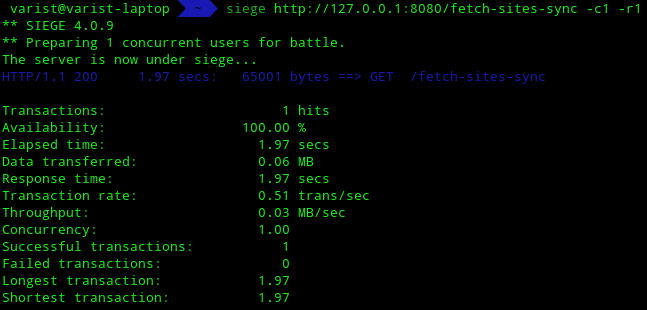
\includegraphics[height=50mm]{zdjecia/1_req_sync_fast}
    \centering
\end{figure}
Zostało wykonane dokładnie jedno zapytanie na endpoint ,,/fetch-sites-sync''. Czas jaki zajęło wykonanie tego zapytania i otrzymania odpowiedzi to 1.89 sekundy, podobnie jak całego procesu wysyłania zapytań i odbierania odpowiedzi.

Aby zobaczyć jak ta sama operacja wykona się w Django w poprzednim poleceniu zmieniamy jedynie port na odpowiadający temu, na którym działa serwis wykonany w Django:
\begin{figure}[H]
    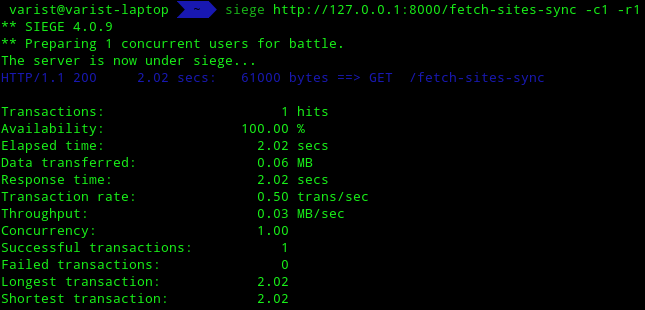
\includegraphics[height=50mm]{zdjecia/1_req_sync_django}
    \centering
\end{figure}

Teraz, aby osiągnąć nieco bardziej reprezentatwyne wyniki zasymulujemy wykonanie tego zapytania przez 10 użytkowników współbieżnie, z których każdy będzie wykonywał po 5 zapytań.
\begin{figure}[H]
    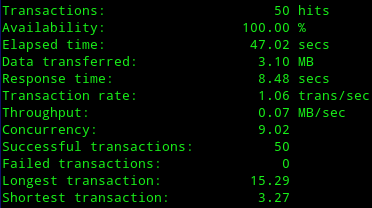
\includegraphics[height=50mm]{zdjecia/10_req_sync_fast}
    \centering
    \caption{FastAPI, 10 użytkowników, 5 zapytań}
\end{figure}

\begin{figure}[H]
    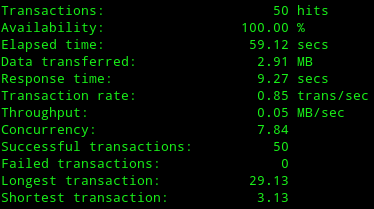
\includegraphics[height=50mm]{zdjecia/10_req_sync_django}
    \centering
    \caption{Django, 10 użytkowników, 5 zapytań}
\end{figure}

Wniosek: Rozbudowanie Django sprawia, że już w wypadku prostego sekwencyjnego wykonania zapytań proces trwa dłużej, gdyż każde zapytanie musi przejść nieco dłuższą drogę. Prawdopodobnym czynnikiem zmniejszającym wydajność Django może być też praca wykonywanay przez klasę JsonResponse, która jest odpowiedzialna za przełożenie otrzymanych odpowiedzi na notację JSON\footnote{JavaScript Object Notation}, jednak spore znaczenie na pewno mają tez wbudowane middleware'y.

\subsection{threading}
Teraz zaczniemy od testu endpointów używających modułu threading od razu używając opcji dziesięciu użytkowników i pięciu zapytań. Zaczynając od FastAPI:
\begin{figure}[H]
    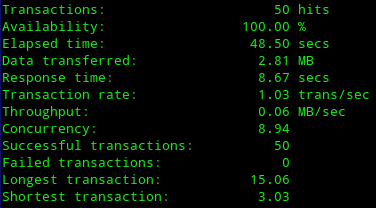
\includegraphics[height=50mm]{zdjecia/10_req_thread_fast}
    \centering
    \caption{FastAPI, threading, 10 użytkowników, 5 zapytań}
\end{figure}

\begin{figure}[H]
    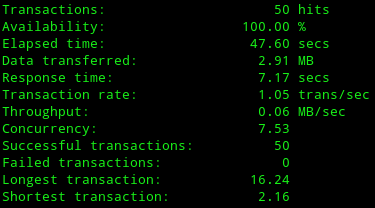
\includegraphics[height=50mm]{zdjecia/10_req_thread_django}
    \centering
    \caption{Django, threading, 10 użytkowników, 5 zapytań}
\end{figure}
Zaobserwować możemy, że przewaga FastAPI, którą widzieliśmy w przykładzie sekwencyjnym tutaj się ulotniła. Związane jest to z mechanizem FastAPI, który decyduje o tym czy widok zdefiniowany jest jako ,,async def'' czy też zwykły ,,def'' przez co w przypadku threadingu oba frameworki wypadają podobnie. Korzystniej wypadałoby użycie widoku zdefiniowanego jako ,,async def'' w FastAPI, jednak w przypadku korzystania z threadingu wewnątrz tak zdefiniowanych widoków rodziłoby się niebezpieczeństwo związane z wyciekami pamięci i zatrzymaniem niektórych wątków, a co za tym idzie utratą części przesłanych danych. Byłoby to rozwiązanie możliwe do implementacji, jeśli możemy pozwolić klientowi naszego api na powtórzenie zapytania w wypadku otrzymania błędu. Należałoby wtedy ocenić korzyści czasowe płynące z zastosowania takiego rozwiązania wobec strat związanych z ponawianiem zapytań.

\subsection{multiprocessing}
\begin{figure}[H]
    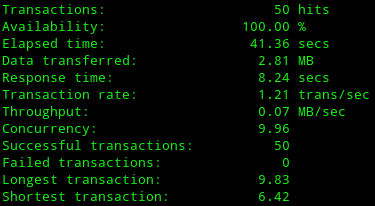
\includegraphics[height=50mm]{zdjecia/10_req_process_fast}
    \centering
    \caption{FastAPI, multiprocessing, 10 użytkowników, 5 zapytań}
\end{figure}

\begin{figure}[H]
    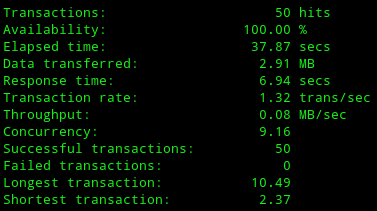
\includegraphics[height=50mm]{zdjecia/10_req_process_django}
    \centering
    \caption{Django, multiprocessing, 10 użytkowników, 5 zapytań}
\end{figure}

Tutaj ponownie przewaga uzyskana przez FastAPI przy klasycznym sekwencyjnym podejściu została zniwelowana. Multiprocessing stanowczo w obu frameworkach działa tak samo dobrze, nawet z lekkim wskazaniem w stronę Django, które przypomnijmy miało być w tym starciu technologią bardziej rozbudowaną, ale jednak wolniejszą. Warto podkreślić, że tak dobry wynik tego rozwiązania nie byłby możliwy bez zastosowania go na architekturze opartej o kilkurdzeniowy procesor.

\subsection{asyncio}
\begin{figure}[H]
    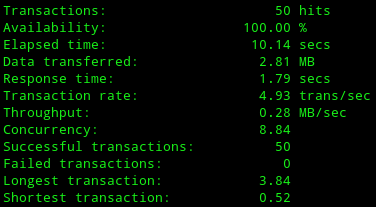
\includegraphics[height=50mm]{zdjecia/10_req_asyncio_fast}
    \centering
    \caption{FastAPI, asyncio, 10 użytkowników, 5 zapytań}
\end{figure}

\begin{figure}[H]
    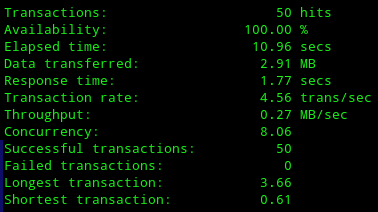
\includegraphics[height=50mm]{zdjecia/10_req_asyncio_django}
    \centering
    \caption{Django, asyncio, 10 użytkowników, 5 zapytań}
\end{figure}
Zgodnie z przewidywaniem technologia asyncio w przypadku tego typu operacji bije konkurencję na głowę. Wzrost wydajności o niemal 40 sekund względem rozwiązania z zastosowaniem threadingu i niemal 30 sekund względem multiprocessingu. Co ciekawe w obu frameworkach czas wykonania jest bardzo zbliżony i różni się o niecałą sekundę. W perspektywie 10 sekund, które zajął cały proces jest to różnica niecałych 10\% na korzyść młodszego frameworka.

\section{Obliczenia}
\subsection{Sekwencyjnie}
Ponownie rozpoczniemy od obejrzenia wyniku wysłania pojedynczego zapytania na endpoint wykonujący przewidywane obliczenia w trybie całkowicie sekwencyjnym.
\begin{figure}[H]
    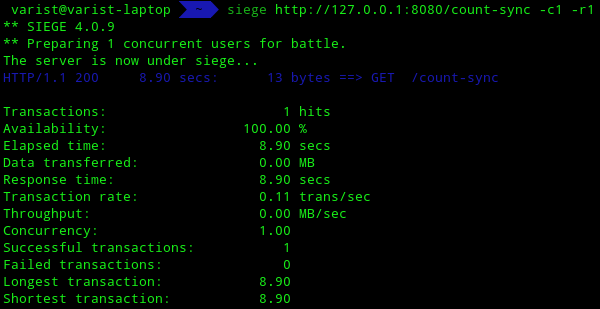
\includegraphics[height=50mm]{zdjecia/1_math_sync_fast}
    \centering
    \caption{FastaAPI, sekwencyjnie, 1 użytkownik, jedno zapytanie}
\end{figure}

\begin{figure}[H]
    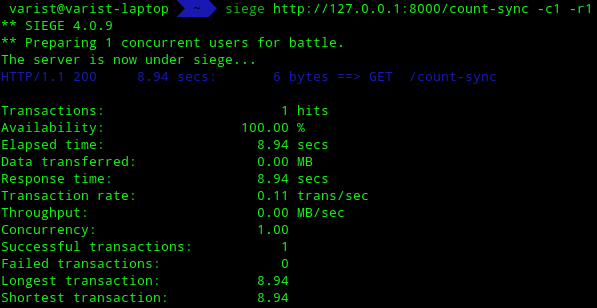
\includegraphics[height=50mm]{zdjecia/1_math_sync_django}
    \centering
    \caption{Django, sekwencyjnie, 1 użytkownik, jedno zapytanie}
\end{figure}
Możemy zaobserwować, że w wypadku obliczeń matematycznych frameworki zachowują się praktycznie identycznie, wynik czasowy różni się o 4 setne sekundy, co przy całkowitym wyniku oscylującym w granicach 8-9 sekund jest wartością pomijalną. Sprawdźmy jednak czy w sytuacji wysłania wielu zapytań sytuacja nie ulegnie zmianie.
\begin{figure}[H]
    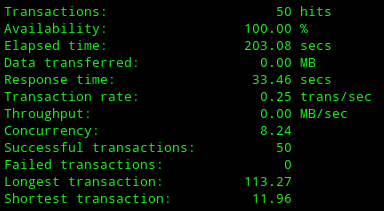
\includegraphics[height=50mm]{zdjecia/10_math_sync_fast}
    \centering
    \caption{FastAPI, sekwencyjnie, 10 użytkowników, 5 zapytań}
\end{figure}

\begin{figure}[H]
    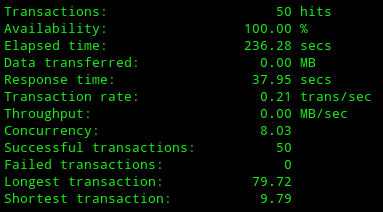
\includegraphics[height=50mm]{zdjecia/10_math_sync_django}
    \centering
    \caption{Django, sekwencyjnie, 10 użytkowników, 5 zapytań}
\end{figure}
Tutaj kwestia wygląda nieco ciekawiej niż w wypadku wysyłania zapytań. Całościowy czas wykonania wszystkich zapytań przez wszystkich użytkowników okazał się być lepszy w wypadku FastAPI - 203 sekundy względem 236 sekund w Django. Co ciekawe jednak zarówno najdłuższy jak i najkrótszy cykl zapytanie-odpowiedź w wypadku FastAPI są znacząco dłuższe niż analogiczne wskaźniki w Django, pomimo że oczywiście średni czas takiego cyklu jest krótszy w FastAPI. Świadczy to o mniej stabilnej pracy wynikowej frameworka i sprawia, że pomimo satysfakcjonującej prędkości jest on w wypadku rozwiązań sekwencyjnych mniej niezawodny.

\subsection{threading}
Zobaczmy jak widoki wykonujące zasobożerne obliczenia będą się zachowywały, gdy do próby ich zrównoleglenia użyjemy threadingu.
\begin{figure}[H]
    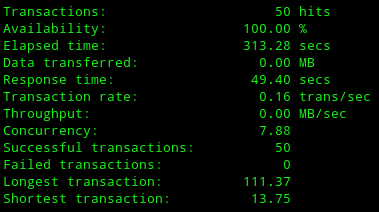
\includegraphics[height=50mm]{zdjecia/10_math_thread_fast}
    \centering
    \caption{FastAPI, threading, 10 użytkowników, 5 zapytań}
\end{figure}

\begin{figure}[H]
    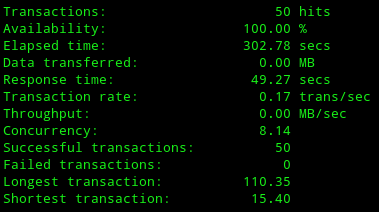
\includegraphics[height=50mm]{zdjecia/10_math_thread_django}
    \centering
    \caption{Django, threading, 10 użytkowników, 5 zapytań}
\end{figure}
W tym przypadku jak widać sytuacja jest dużo bardziej zbliżona. Czasowo ze wszystkimi zapytaniami lepiej poradziło sobie Django, jednocześnie nieco lepiej wypadając również w kwestii najrótszego oraz nadłuższego zapytania. Choć różnica tutaj nie jest tak duża, to jednak zaskakującym jest, że ponownie znajduje się aspekt, w którym starszy framework radzi sobie lepiej.

\subsection{multiprocessing}
Warto nadmienić, że według oczekiwań multiprocessing powinien być rozwiązaniem, które w przypadku wykonywania obliczeń matematycznych powinien w środowisku wielordzeniowym poradzić sobie najlepiej. Sprawdźmy czy to przewidywanie jest słuszne.
\begin{figure}[H]
    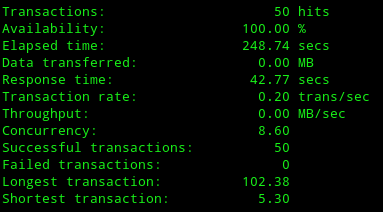
\includegraphics[height=50mm]{zdjecia/10_math_process_fast}
    \centering
    \caption{FastAPI, multiprocessing, 10 użytkowników, 5 zapytań}
\end{figure}

\begin{figure}[H]
    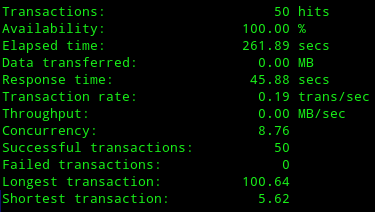
\includegraphics[height=50mm]{zdjecia/10_math_process_django}
    \centering
    \caption{Django, multiprocessing, 10 użytkowników, 5 zapytań}
\end{figure}
Multiprocessing poradził sobie widocznie lepiej niż threading. Wzrost prędkości jest między tymi dwoma rozwiązaniami wyraźny, jednak ciekawą obserwacją jest to, że multiprocessing wypadł słabiej niż rozwiązanie sekwencyjne korzystające z jednego wątku. Wyjaśnienie takiego stanu rzeczy jest dość proste. Stosując rozwiązanie jakim jest serwer gunicorn włączane są cztery procesy - parametr -w wskazuje nam jaka dokładnie liczba workerów powinna pracować cały czas. Oznacza to że w zasadzie już z założenia gunicorna nasza aplikacja jest aplikacją wieloprocesową, a dodanie dodatkowych procesów wewnątrz endpointa powoduje jedynie dodatkowy narzut jaki system musi wykonać by nimi zarządzać. Sytuacja oczywiście byłaby inna, gdybyśmy dysponowali maszyną o bardzo wielu rdzeniach, lecz przy naszym zastosowaniu - warto pomyśleć o innym rozwiązaniu.

\subsection{asyncio}
\begin{figure}[H]
    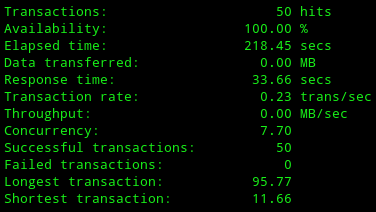
\includegraphics[height=50mm]{zdjecia/10_math_asyncio_fast}
    \centering
    \caption{FastAPI, asyncio, 10 użytkowników, 5 zapytań}
\end{figure}

\begin{figure}[H]
    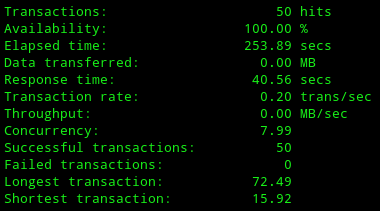
\includegraphics[height=50mm]{zdjecia/10_math_asyncio_django}
    \centering
    \caption{Django, asyncio, 10 użytkowników, 5 zapytań}
\end{figure}
Już szybki rzut oka na powyższe wyniki pozwala nam odczytać, że niekwestionowanym zwycięzcą spośród naszych mechanizmów zrównoleglania jest asyncio. Bez wątpienia jest to technologia, która w naszym przypadku użycia spisała się najlepiej, wciąż jednak nieco gorzej niż rozwiązanie sekwencyjne. Ponadto dużo lepiej w użyciu asyncio wypadło FastAPI - różnica aż o około 20\% sprawia, że jeśli chcieć używać asynchroniczności w kontekście aplikacji webowych - FastAPI powinno być naszym pierwszym wyborem.

\section{Wnioski}

Podsumowując przeprowadzone we wcześniej części tego rozdziału testy stworzyłem następującą tabelę prezentującą wyniki czasowe widoków wysyłających zapytania. Widać tutaj lekką przewagę nieco bardziej doświadczonego frameworka jakim jest Django, jednak przewaga ta jest widoczna jedynie w technologiach uruchamianych w kontekście sekwencyjnym, a także tam gdzie używane są mechanizmy threading oraz multiprocessing. Już natomiast w wypadku użycia asyncio przewaga zmienia się na korzyść nowocześniejszego frameworka. 

\begin{table}[ht]
\caption{Wyniki czasowe wysyłania zapytań}
\centering
\begin{tabular}{c c c c}
\hline\hline
Mechanizm & FastAPI & Django \\ [0.5ex]

\hline
Sekwencyjnie & 47.02s & 59.12s \\
threading & 48.50s & 47.60s \\
multiprocessing & 41.36 & 37.87s \\
asyncio & 10.14 & 10.96s \\[1ex]
\hline
\end{tabular}
\end{table}

Druga tabela w tej części to już wyniki podsumowujące pracę frameworków w kontekście wykonywania pracy obliczeniowej związanej z Centralną Jednostką Obliczeniową naszego serwera.
\begin{table}[ht]
\caption{Wyniki czasowe obliczeń}
\centering
\begin{tabular}{c c c c}
\hline\hline
Mechanizm & FastAPI & Django \\ [0.5ex]

\hline
Sekwencyjnie & 203.08s & 236.28s \\
threading & 313.28s & 302.78s \\
multiprocessing & 248.74 & 261.89s \\
asyncio & 218.45s & 253.89s \\[1ex]
\hline
\end{tabular}
\end{table}

Tutaj jak już wspominałem wyniki są dość zaskakujące. Sporą część pracy, którą w normalnej sytuacji wykonywałyby mechanizmy zrównoleglające - tutaj wykonywana jest przez workery, którymi posługuje się nasza aplikacja.

W tym przypadku również różnica między frameworkami nie jest tak oczywista - pomimo użycia dokładnie tych samych parametrów wyniki czasowe są zróżnicowane. W rozwiązaniu sekwencyjnym lepiej z rozporządzaniem mocą obliczeniową poradziło sobie FastAPI, przy użyciu threadingu niewielką przewagę uzyskało Django, zaś odwrotna sytuacja zaistniała w przypadku multiprocessingu. Niekwestionowanym słusznym rozwiązaniem w przypadku użycia asyncio jest framework FastAPI - tutaj sytuacja jest bardzo zbliżona do opcji z części wysyłającej zapytania i nie ma wątpliwości, że jeśli przy projektowaniu architektury naszego programu wiemy, że będziemy korzystać z asynchronicznych funkcjonalności Pythona to nasz wybór powinien paść na FastAPI, w przeciwnym wypadku zaś - skłonić się powinniśmy ku Django.